\documentclass[10pt,pdf,aspectratio=169]{beamer}
\usepackage[T1,T2A]{fontenc}
% Входная кодировка utf-8
\usepackage[utf8]{inputenc}
% Поддержка русского и английского. В частности переносы
\usepackage[english,russian]{babel}

% Theme for beamer presentation.
\usepackage{beamerthemesplit}
% Other themes include: beamerthemebars, beamerthemelined,
%                       beamerthemetree, beamerthemetreebars

\newcommand{\inp}[1]{\input{../../out/#1}}
\newcommand{\characteristic}[2]{\inp{#1/characteristics/#2}}
\newcommand{\descriptive}[2]{\inp{#1/descriptive/#2}}
\newcommand{\test}[3]{\inp{#1/test/#2/#3}}
\newcommand{\normaldistr}{$\mathcal{N}(\descriptive{original}{mean}, \descriptive{original}{variance})$}

\logo{
\includegraphics[width=1cm,height=1cm,keepaspectratio]{Logo_BSU.jpg}}
\title[Анализ и прогнозирование гидрологических данных]{Анализ и прогнозирование гидрологических данных}    % Enter your title between curly braces
\author[Павлов Александр]{Павлов Александр Сергеевич}                 % Enter your name between curly braces
\institute{Кафедра Теории Вероятностей и Математической Статистики}      % Enter your institute name between curly braces
\date{\today}                    % Enter the date or \today between curly braces

\begin{document}

% Creates title page of slide show using above information
\begin{frame}
  \titlepage
\end{frame}

% \section[План]{}

% % Creates table of contents slide incorporating
% % all \section and \subsection commands
% \begin{frame}
%   \tableofcontents
% \end{frame}


\section{}

\begin{frame}
  \frametitle{Постановка задачи}   % Insert frame title between curly braces

  \begin{itemize}
    \item Первичный анализ данных
    \item Корреляционный анализ
    \item Анализ остатков
    \item Регрессионный анализ
    \item Вариограммный анализ
    \item Прогнозирование методом Кригинга
  \end{itemize}
\end{frame}

\section{Первичный анализ}


\begin{frame}
  \frametitle{Исходные данные}   % Insert frame title between curly braces
  \begin{columns}[c]
  \column{2in}  % slides are 3in high by 5in wide
  Исходные данные получены от учебно-научного центра <<Нарочанская биологическая станция им. Г.Г.Винберга>> .

  На рисунке представлена выборка наблюдений за температурой воды в июле месяце в период с 1975 по 2012 годы.
  \column{3in}
  \framebox{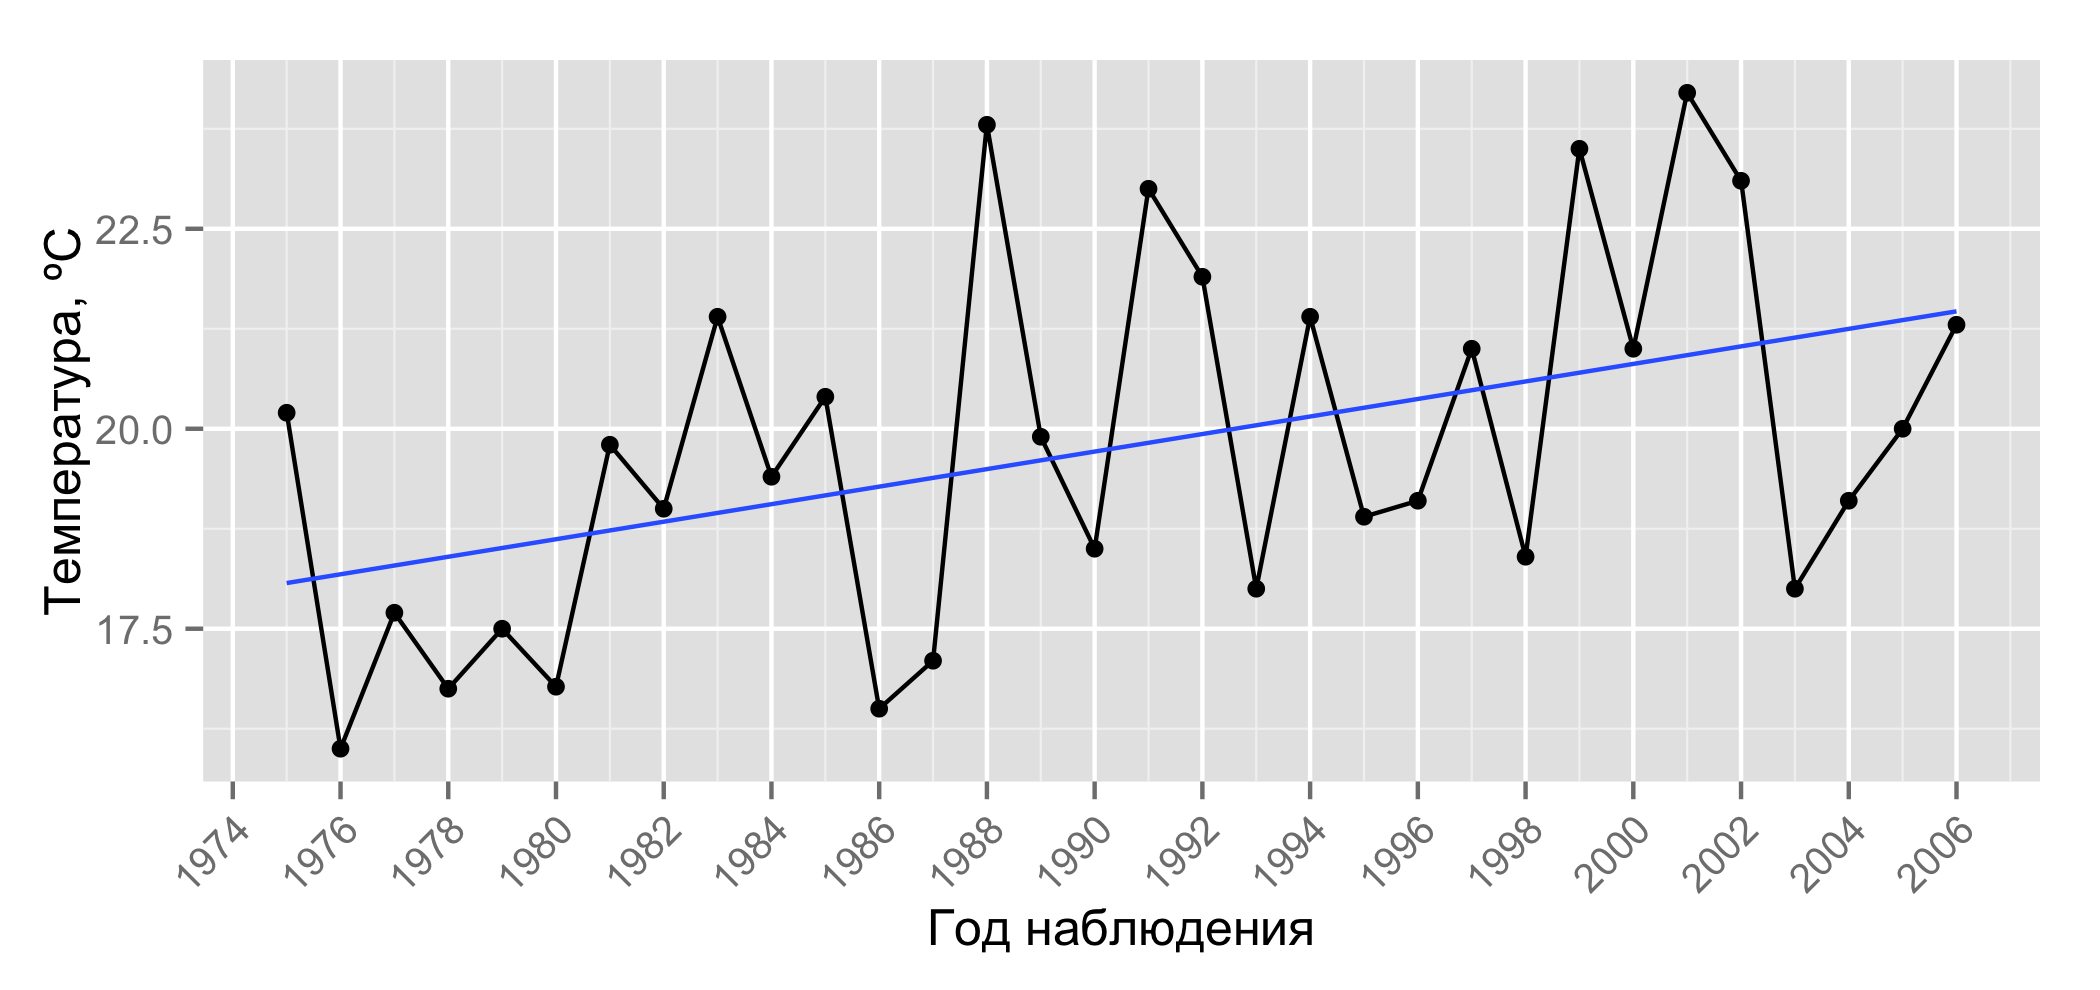
\includegraphics[width=3in]{../../figures/original/time-series.png}
  }
  \end{columns}
\end{frame}

\subsection{Описательные статистики}

\begin{frame}
  \frametitle{Основные описательные статистики}   % Insert frame title between curly braces

  % latex table generated in R 3.1.2 by xtable 1.7-4 package
% Fri May 15 14:18:49 2015
\begin{table}[ht]
\centering
\begin{tabular}{rr}
  \hline
 & Значение \\ 
  \hline
Среднее & 19.88 \\ 
  Медиана & 19.80 \\ 
  Нижний квартиль & 18.20 \\ 
  Верхний квартиль & 21.40 \\ 
  Минимум & 16.00 \\ 
  Максимум & 24.20 \\ 
  Размах & 8.20 \\ 
  Квартильный размах & 3.20 \\ 
  Дисперсия & 4.92 \\ 
  Стандартное отклонение & 2.22 \\ 
  Коэффициент вариации & 24.75 \\ 
  Стандартная ошибка & 0.37 \\ 
  Асимметрия & 0.18 \\ 
  Ошибка асимметрии & 0.40 \\ 
  Эксцесс & -0.79 \\ 
  Ошибка эксцесса & 0.78 \\ 
   \hline
\end{tabular}
\caption{Описательные статистики для наблюдаемых температур.} 
\label{table:dstats}
\end{table}


\end{frame}

\subsection{Проверка на нормальность}

\begin{frame}
  \frametitle{Гистограмма наблюдаемых температур}   % Insert frame title between curly braces
   \begin{columns}[c]
   \column{4.5in}
  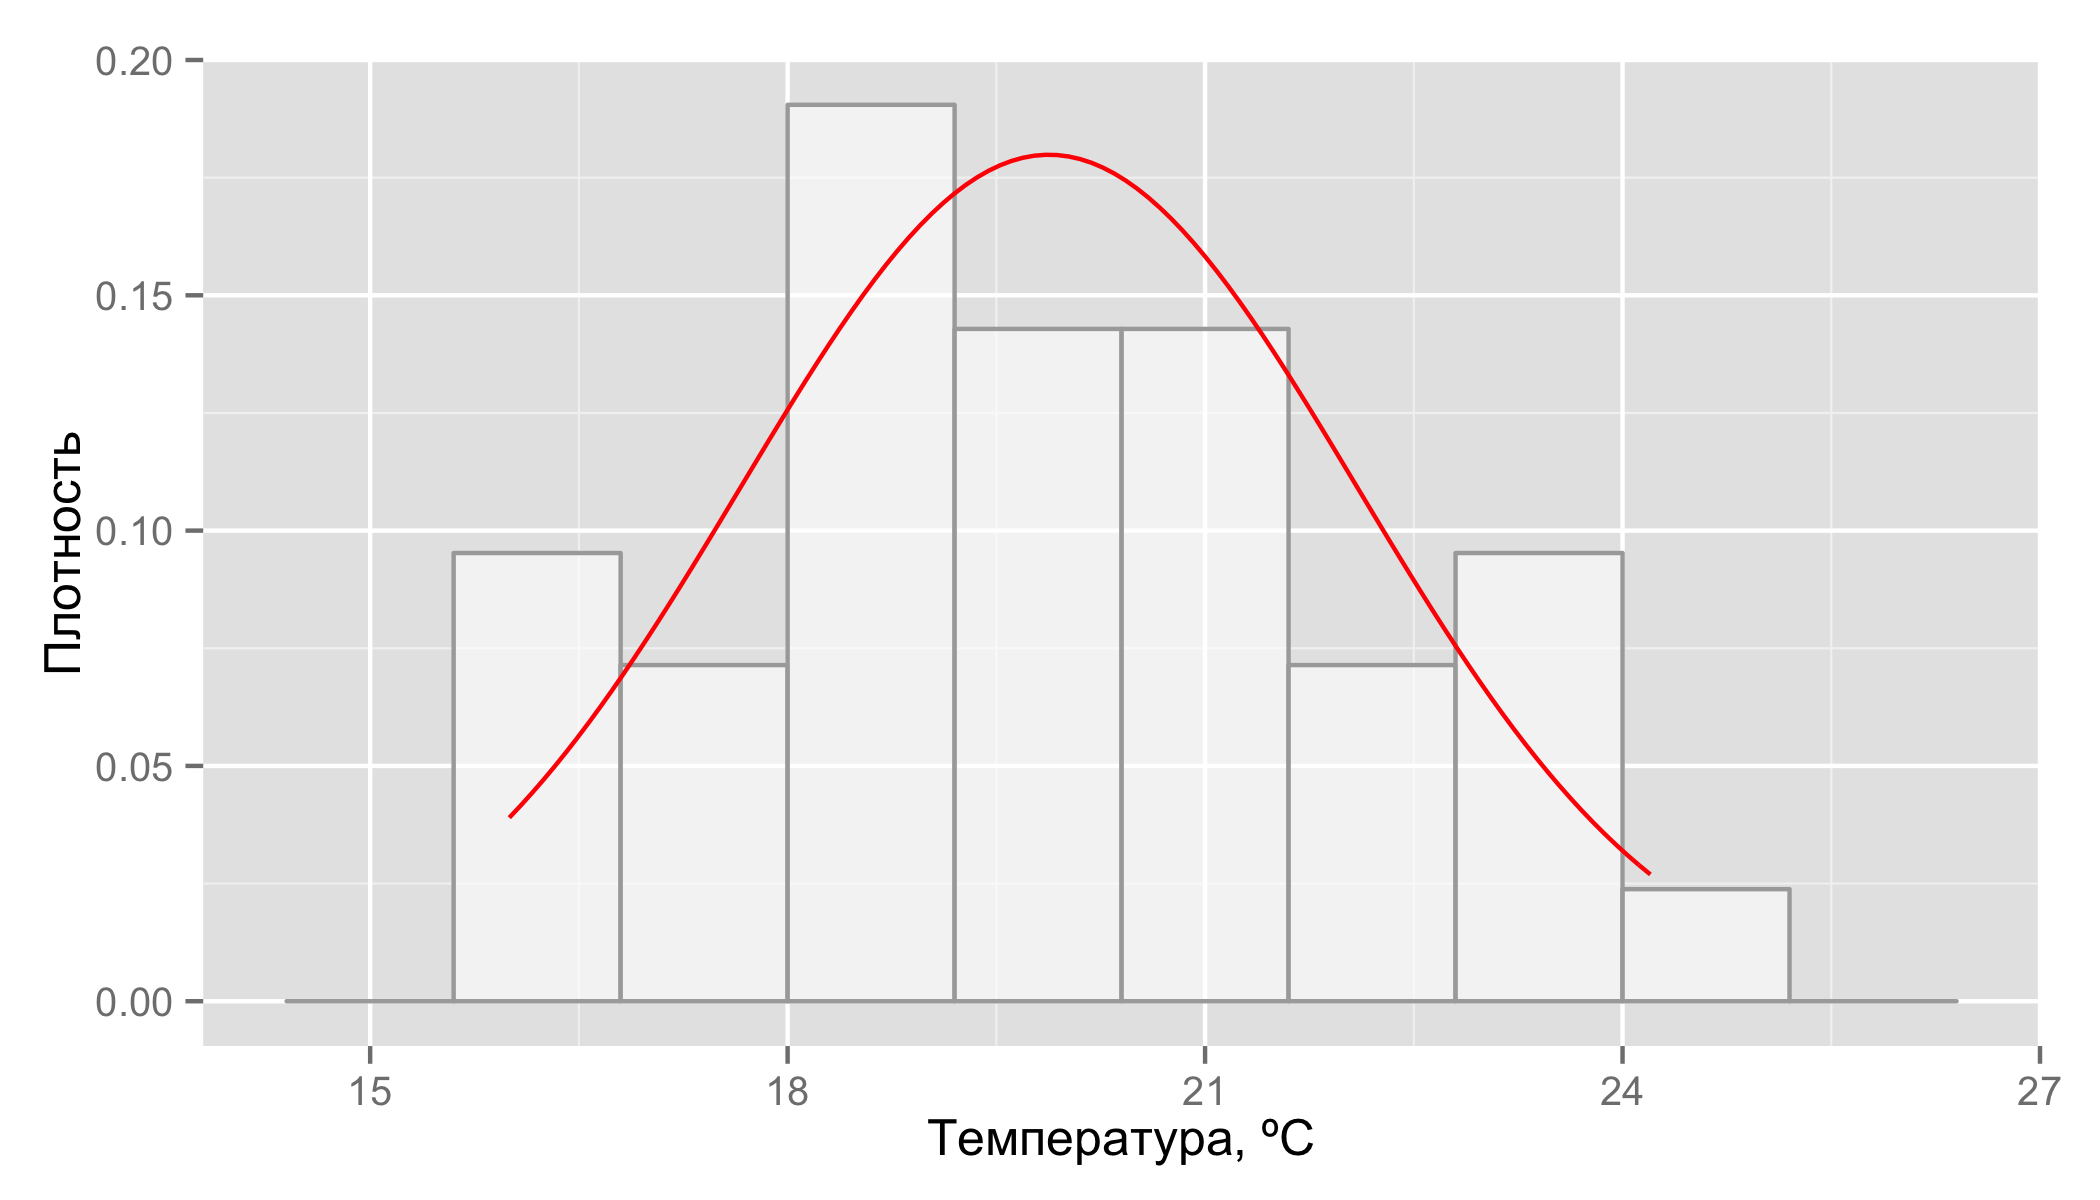
\includegraphics[width=4.5in]{../../figures/original/histogram.png}
  \end{columns}
\end{frame}

\begin{frame}
  \frametitle{График квантилей}   % Insert frame title between curly braces
   \begin{columns}[c]
   \column{4.5in}
  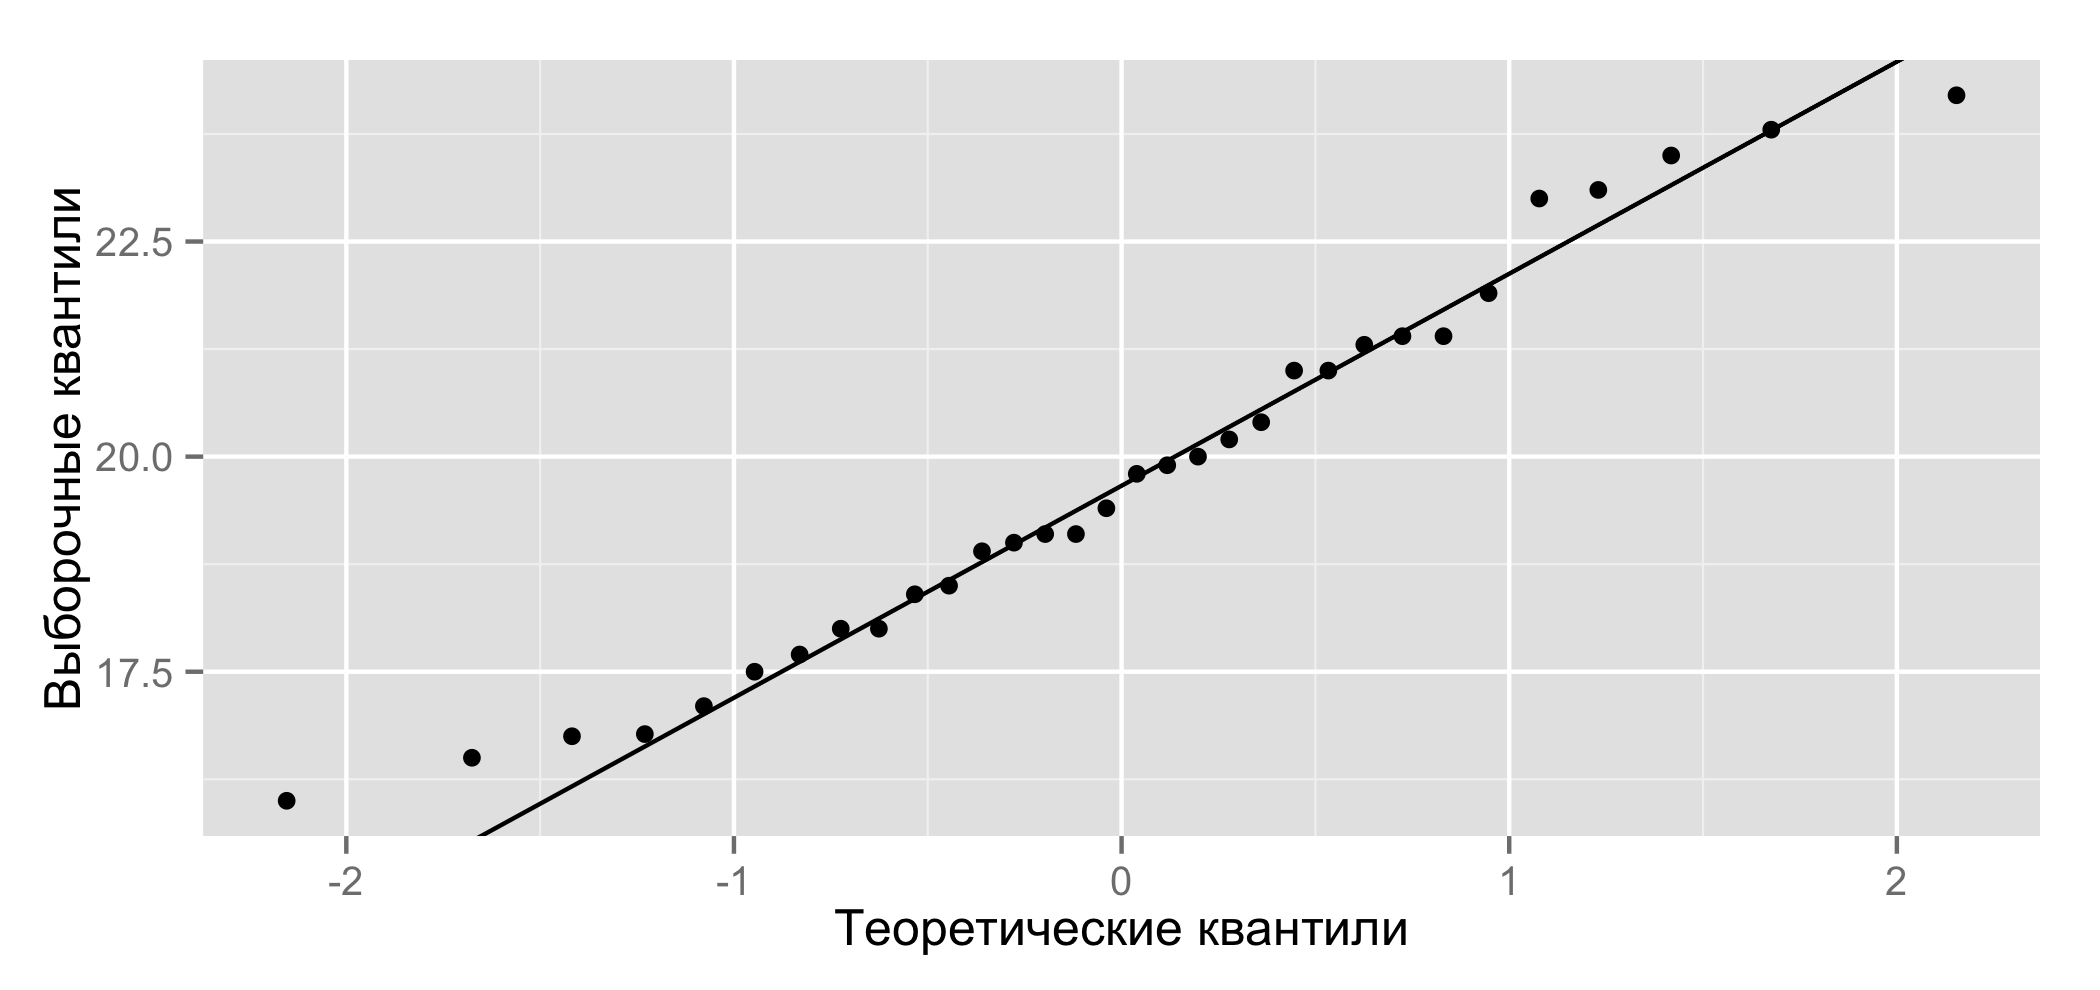
\includegraphics[width=4.5in]{../../figures/original/quantile.png}
  \end{columns}
\end{frame}

\section{Корреляционный анализ}

\subsection{Проверка наличия зависимости между температурой воды и временем}
\begin{frame}
  \frametitle{Диаграмма рассеяния}   % Insert frame title between curly braces
  \begin{columns}[c]
  \column{2in}  % slides are 3in high by 5in wide
  \begin{itemize}
  \item<1-> Выборочный коэффициент корреляции: $ r_{xt} = \characteristic{original}{correlation} $
  \item<2-> При уровне значимости $ \alpha=0.05 $ выборочный коэффициент является значимым
  \end{itemize}
  \column{3in}
  \framebox{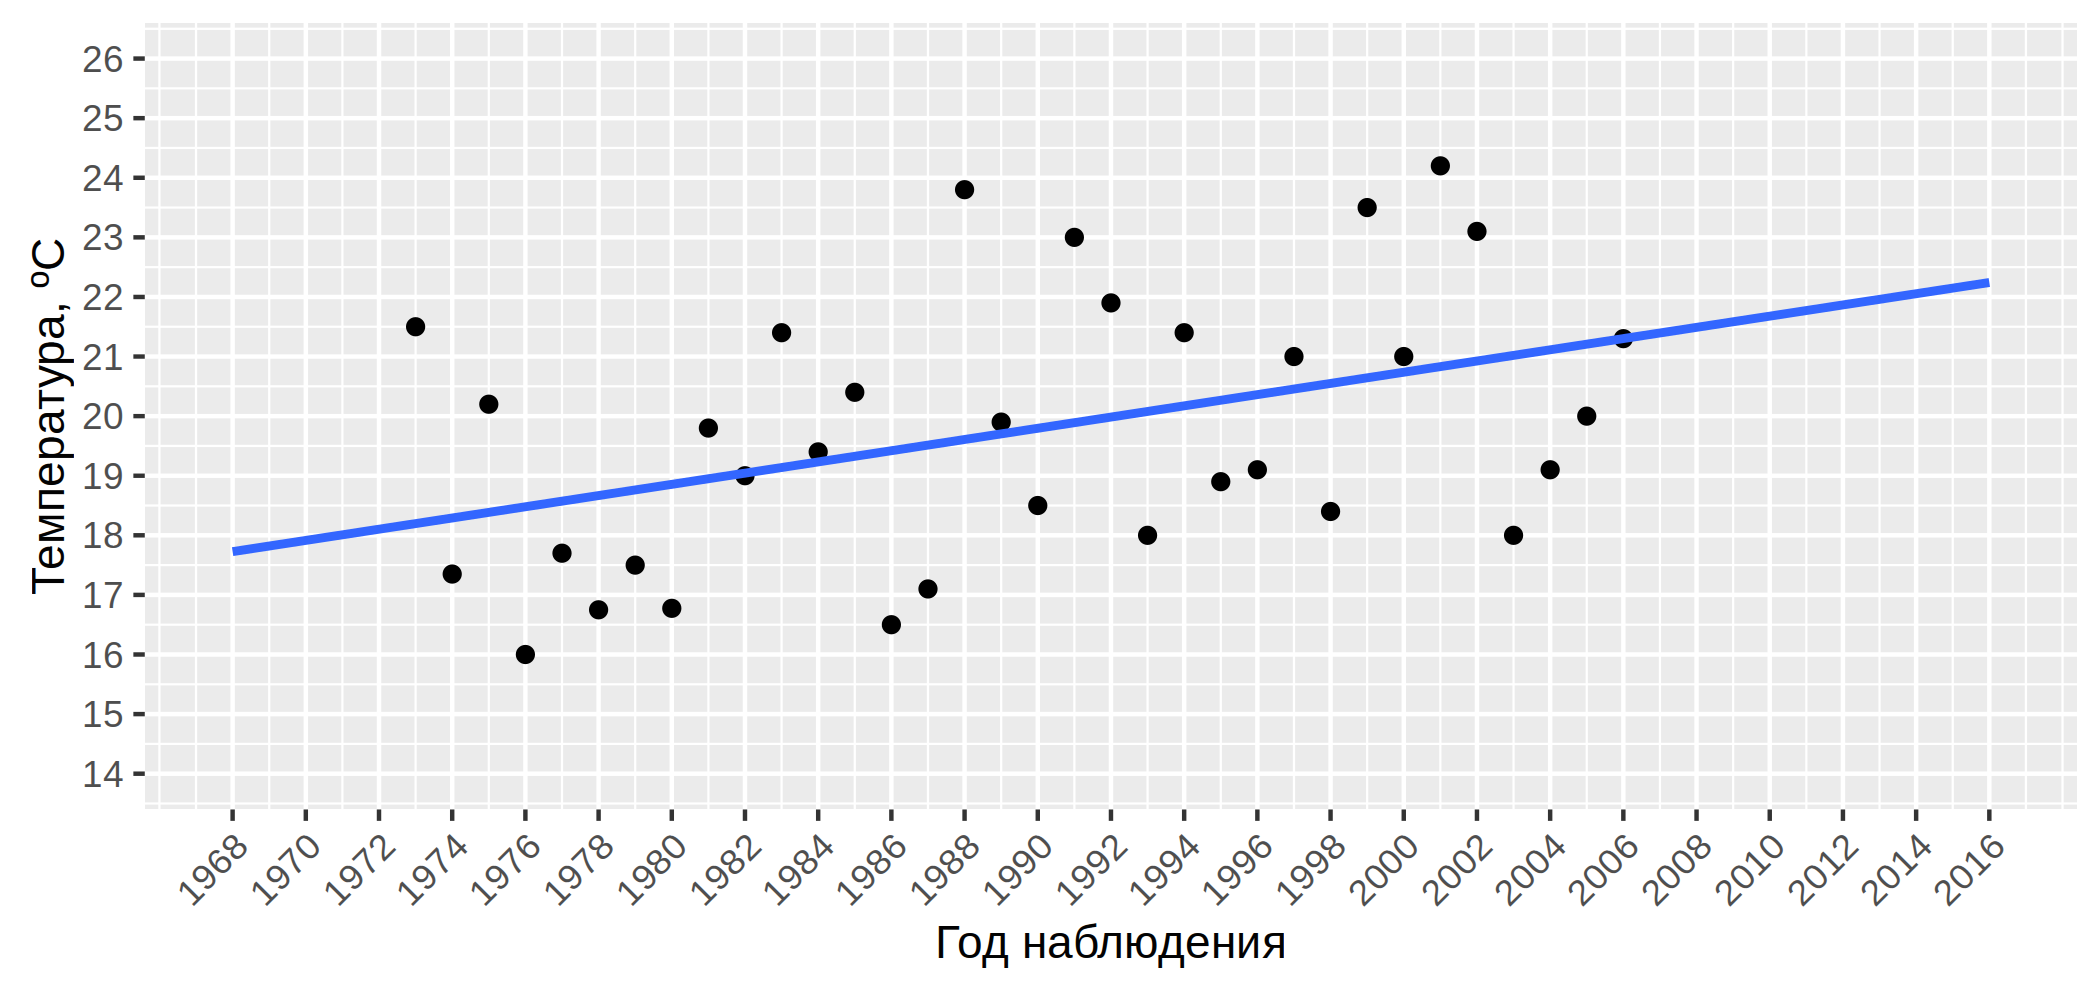
\includegraphics[width=3in]{../../figures/original/scatterplot.png}}
  \end{columns}
\end{frame}

\section{Регрессионный анализ}

\subsection{Регрессионная модель}
\begin{frame}
  \frametitle{Временной ряд}   % Insert frame title between curly braces
  \begin{columns}[c]
  \column{2in}  % slides are 3in high by 5in wide
  \begin{itemize}
  \item<1-> Модель временного ряда: $ X = T + E $
  \item<2-> Уравнение тренда: $ x(t) = at + b = 0.1014t + 18.0521 $
  \end{itemize}
  \column{3in}
  \framebox{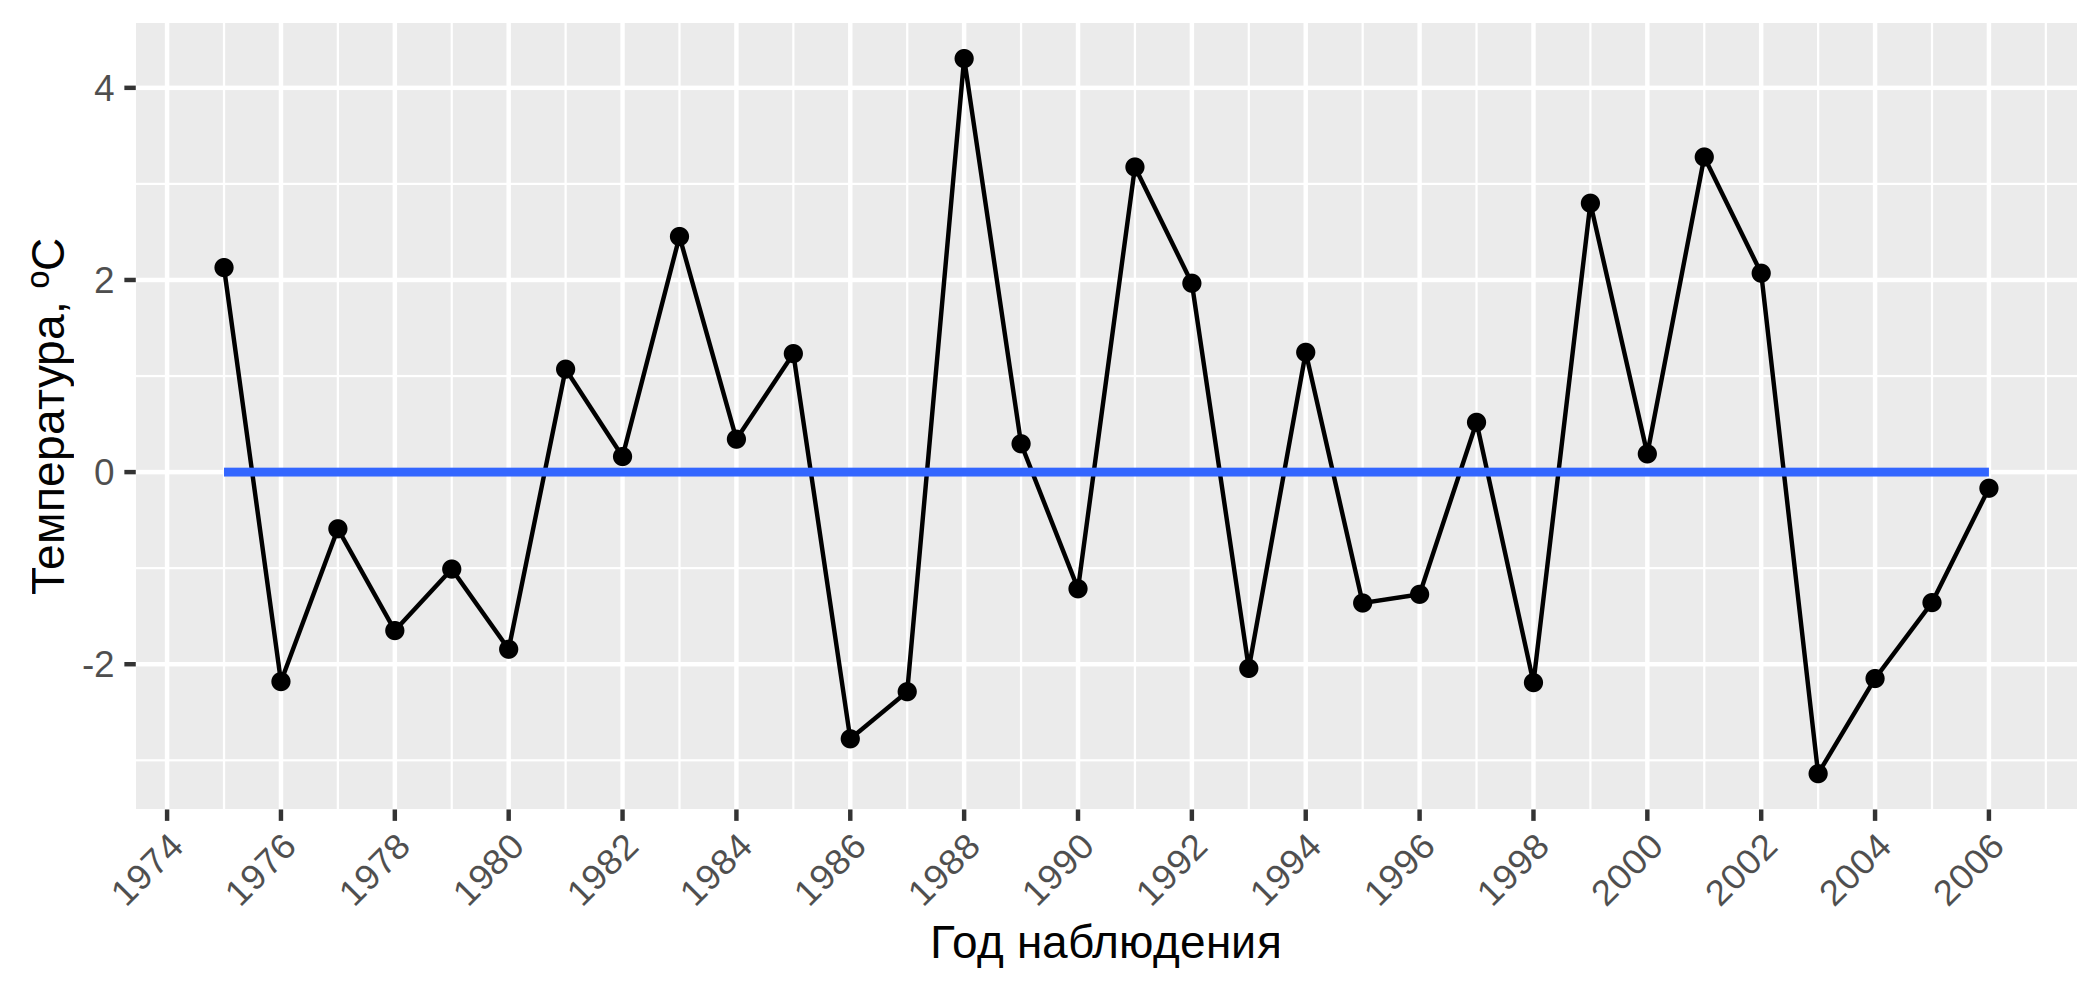
\includegraphics[width=3in]{../../figures/residual/time-series.png}}
  \end{columns}
\end{frame}

\subsection{Качество регрессионной модели}
\begin{frame}
  \frametitle{Оценка модели}   % Insert frame title between curly braces
  \begin{itemize}
    \item<1-> С помощью критерия Стьюдента доказана значимость коэффициентов регрессионной модели
    \item<2-> F-критерий Фишера при уровне значимости $ \alpha = 0.05 $ показал адекватность модели
    \item<3-> Точность модели невысока, посколько коэффициент детерминации $ \eta^2_{x(t)} = 0.275 $
  \end{itemize}
\end{frame}

\subsection{Анализ остатков}

\begin{frame}
  \frametitle{Автокорреляционная функция}   % Insert frame title between curly braces
   \begin{columns}[c]
   \column{4.5in}
  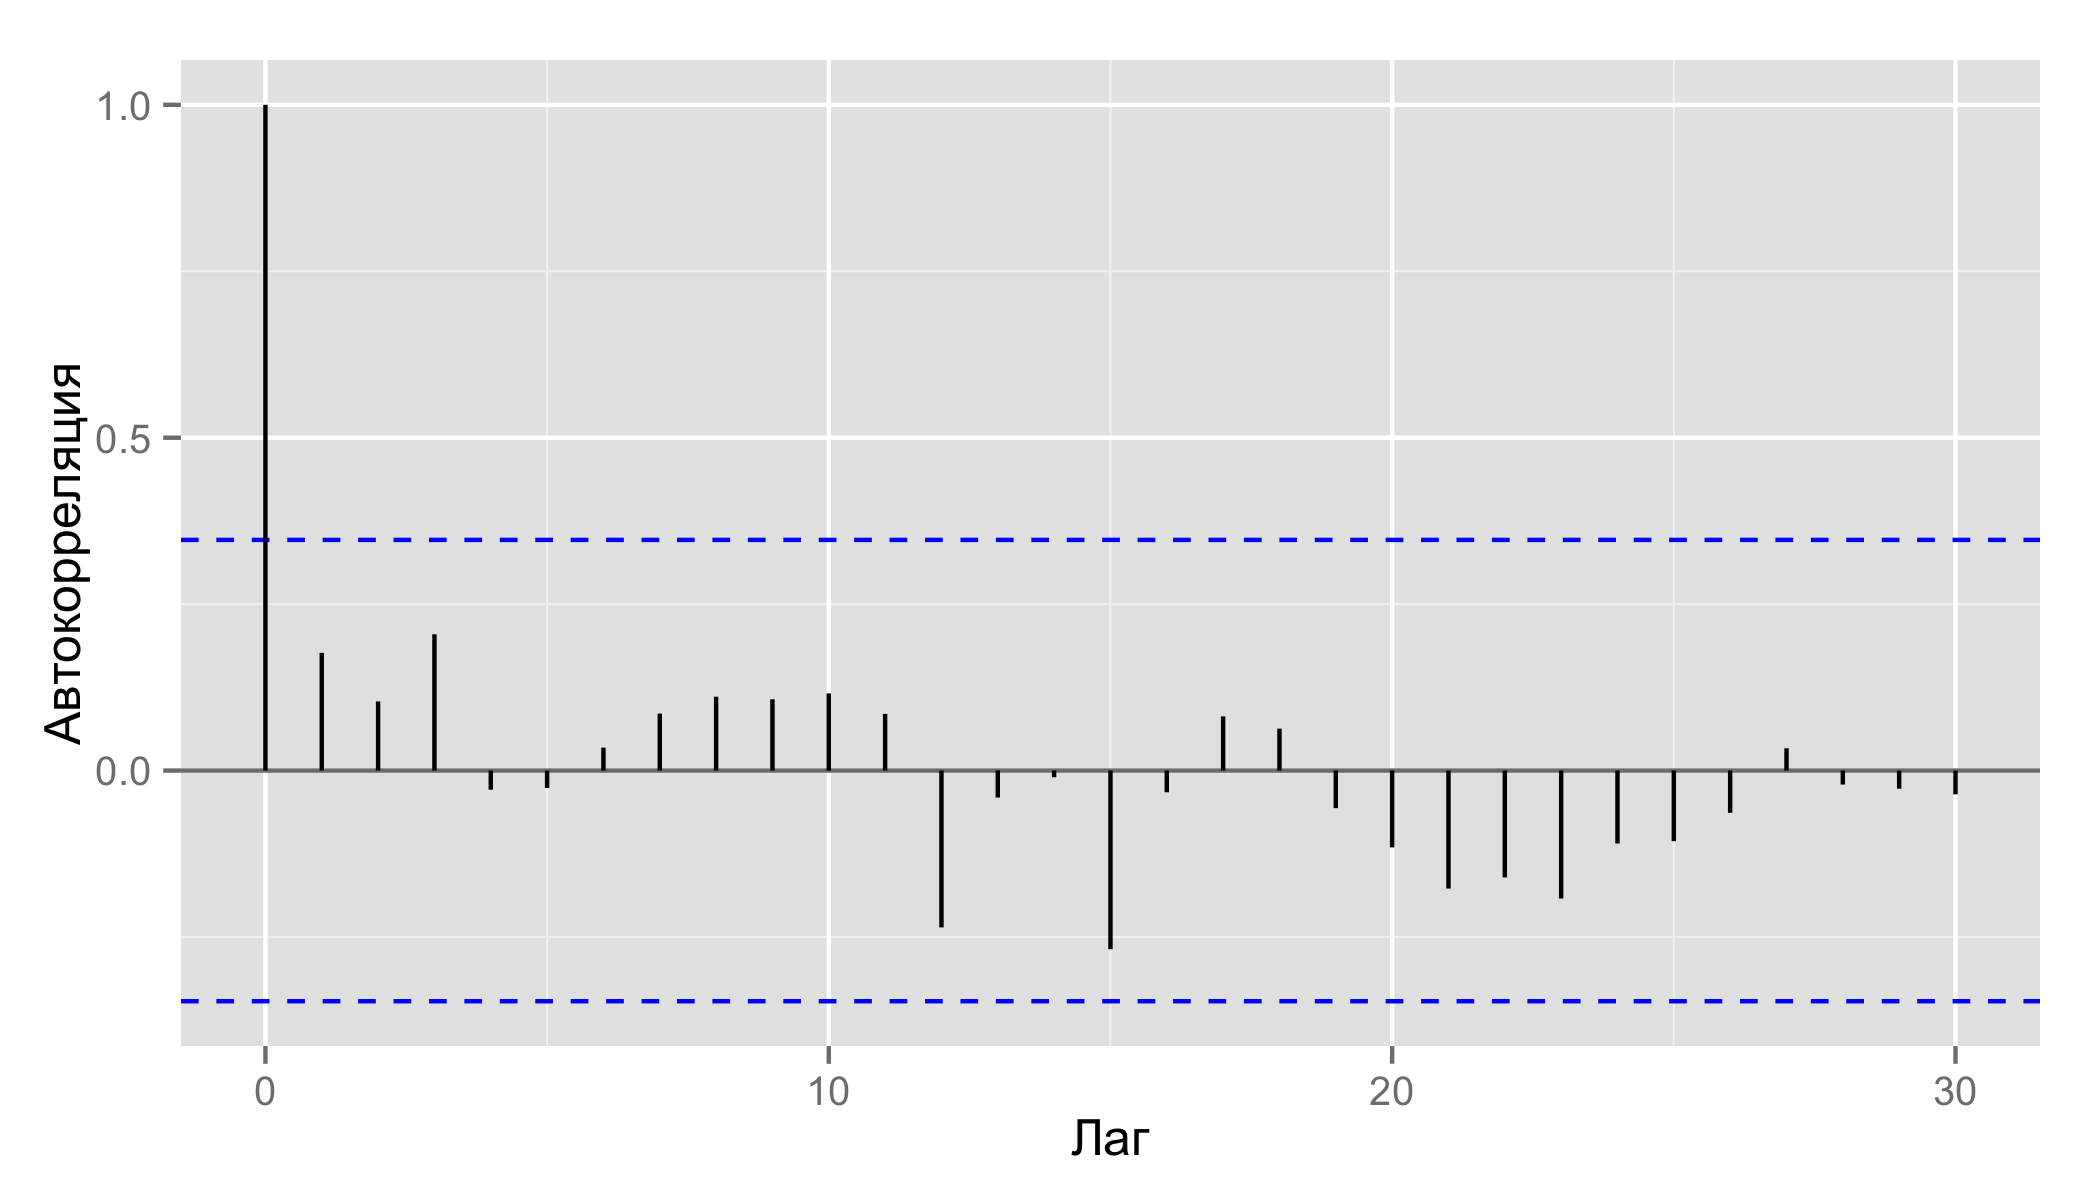
\includegraphics[width=4.5in]{../../figures/residual/acf.png}
  \end{columns}
\end{frame}

\section{Вариограммный анализ}

\subsection{Вариограмма}

\begin{frame}
  \frametitle{График экспериментальной вариограммы}   % Insert frame title between curly braces
   \begin{columns}[c]
   \column{4.5in}
  % \includegraphics[width=4.5in]{../../figures/article/variog1.png}
  \end{columns}
\end{frame}

\begin{frame}
  \frametitle{График экспериментальной вариограммы с подобранной моделью}   % Insert frame title between curly braces
  \begin{columns}[c]
  \column{2in}  % slides are 3in high by 5in wide
  Параметры модели:
  \begin{itemize}
  \item Модель: Сферическая с эффектом самородков
  \item Эффект самородков: $3.82$
  \item Порог: $4.22$
  \item Ранг: $4.19$
  \end{itemize}
  \column{3in}
  % \framebox{\includegraphics[width=3in]{../../figures/article/variog.png}}
  \end{columns}
\end{frame}

\subsection{Кригинг}
\begin{frame}
  \frametitle{Прогнозирование методом ординарного кригинга}   % Insert frame title between curly braces
   \begin{columns}[c]
   \column{4.5in}
  % \includegraphics[width=4.5in]{../../figures/article/actvspredpred.png}
  \end{columns}
\end{frame}

% \subsection{}
% \begin{frame}
%   \frametitle{}   % Insert frame title between curly braces
%    \begin{columns}[c]
%    \column{1.3in}
%   Спасибо за внимание
%   \end{columns}
% \end{frame}
\end{document}